\section{El simulador}

Anam a definir com està organitzat el nostre simulador.

\paragraph{Esdeveniments}

\begin{enumerate}

  \item Tasca d'usuari: un usuari ha acabat de reflexionar i llança una tasca
    cap a la CPU.

  \item Sortida de la CPU: una transacció surt de la CPU i pot anar al disc o
    tornar a reflexionar. Aquesta decisió està codificada estadísticament
    segons el nombre de peticions a disc per transacció.

  \item Sortida del disc: una transacció del disc sempre passa per la CPU.

\end{enumerate}

\paragraph{Variables d'estat}

\begin{enumerate}

  \item Rellotge global

  \item Instant de sortida d'una tasca

  \item Instant d'arribada d'una tasca

\end{enumerate}

\paragraph{Variables estadístiques}

\begin{enumerate}

  \item Temps de processament acumulat, necessari per calcular els temps de
    processament mig.

  \item Nombre de repeticions totals.

\end{enumerate}

\subsection{Organització interna}

El simulador consta de varis mòduls:

\begin{description}

  \item[Principal] coordinador entre els distints mòduls. Està programat al
    fitxer \verb+main.py+ i \verb+sim.py+.

  \item[Inicialitzador] posa a zero els valors i omple de tasques els servidors
    dels usuaris. Està adins el \verb+sim.py+.

  \item[Temporització] mitjançant una cua de prioritats gestiona els distints
    esdeveniments i calcula el següent a llançar. També està a \verb+sim.py+.

  \item[Esdeveniments] genera la resposta a un esdeveniment escollit per la
    temporització. Es troba dins el model de cada servidor, a \verb+model.py+.

  \item[Aleatoris] ampliació del mòdul escrit a PL1 per cobrir les
    distribucions contants i exponencials, al \verb+rand.py+.

  \item[Informe] ajuda a determinar el final de la simulació. També genera els
    càlculs estadístics i les gràfiques. Són els mòduls \verb+statistic.py+,
    \verb+suite.py+ i \verb+chart_generation.py+.

\end{description}

El diagrama de blocs es troba generalitzat al gràfic
~\ref{sim:fig:diagrama-moduls}.

\begin{figure}
  \centering
  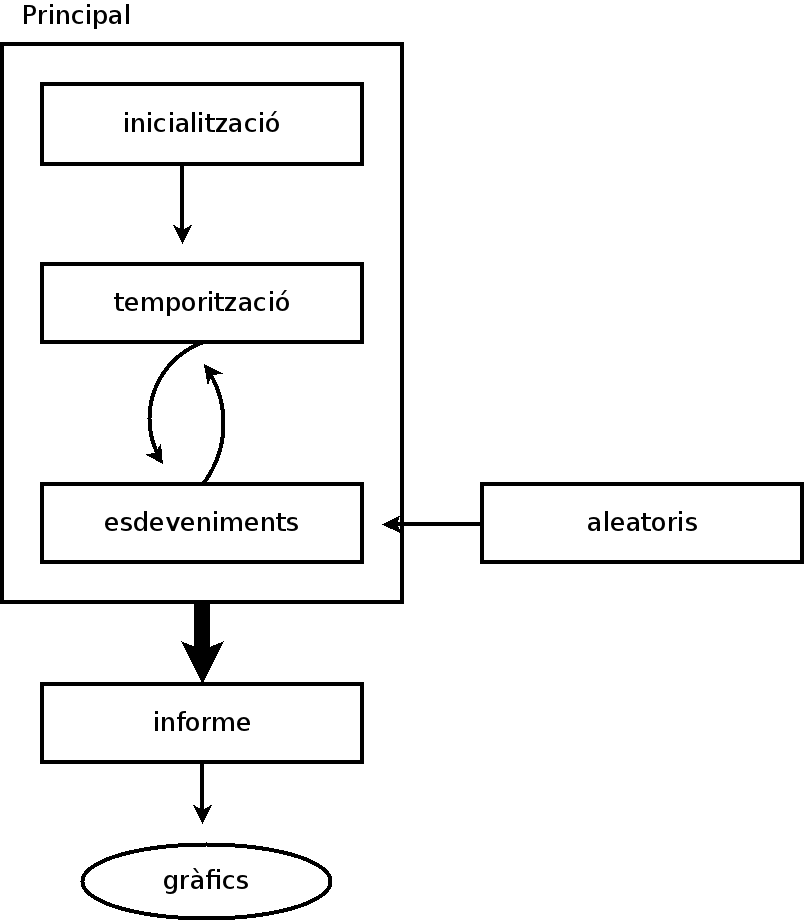
\includegraphics[width=\textwidth]{img/diagrama-moduls.png}
  \caption{Diagrama de mòduls del simulador.}
  \label{sim:fig:diagrama-moduls}
\end{figure}

\section{Pseudocodi}

El pseudocodi del simulador el podem trobar a la figura
~\ref{sim:codi:pseudocodi}.

\begin{figure}
  \centering
  \pycode{pseudocodi}
  \caption{Pseudocodi general del simulador.}
  \label{sim:codi:pseudocodi}
\end{figure}


\section{Desenvolupament}

Sobre el desenvolupament real del simulador cal dir:

\begin{enumerate}

  \item S'ha programat amb el llenguatge de propòsit general Python.

  \item No s'ha duit a terme la validació amb QNAP2.

  \item Per determinar el tamany del transitori s'han fet distintes proves amb
    la durada de la simulació. Llavors hem tallat considerant la primera meitat
    dels esdeveniments transitori.

  \item S'han fet un mínim de 50 rèpliques per variable de nombre de clients i
    llavors se n'han fet tantes com ha calgut per obtenir una desviació de
    manco el 0,1.

\end{enumerate}
